% GNUPLOT: LaTeX picture with Postscript
\documentclass{minimal}
% Set font size
\makeatletter
\def\@ptsize{1}
\InputIfFileExists{size11.clo}{}{%
   \GenericError{(gnuplot) \space\space\space\@spaces}{%
      Gnuplot Error: File `size11.clo' not found! Could not set font size%
   }{See the gnuplot documentation for explanation.%
   }{For using a font size a file `size<fontsize>.clo' has to exist.
        Falling back ^^Jto default fontsize 10pt.}%
  \def\@ptsize{0}
  \input{size10.clo}%
}%
\makeatother
% Load packages
\usepackage{calc}
\usepackage{graphicx}
\usepackage{color}
\makeatletter
% Select an appropriate default driver (from TeXLive graphics.cfg)
\begingroup
  \chardef\x=0 %
  % check pdfTeX
  \@ifundefined{pdfoutput}{}{%
    \ifcase\pdfoutput
    \else
      \chardef\x=1 %
    \fi
  }%
  % check VTeX
  \@ifundefined{OpMode}{}{%
    \chardef\x=2 %
  }%
\expandafter\endgroup
\ifcase\x
  % default case
  \PassOptionsToPackage{dvips}{geometry}
\or
  % pdfTeX is running in pdf mode
  \PassOptionsToPackage{pdftex}{geometry}
\else
  % VTeX is running
  \PassOptionsToPackage{vtex}{geometry}
\fi
\makeatother
% Set papersize
\usepackage[papersize={680.30bp,396.80bp},text={680.30bp,396.80bp}]{geometry}
% No page numbers and no paragraph indentation
\pagestyle{empty}
\setlength{\parindent}{0bp}%
% Load configuration file
\InputIfFileExists{gnuplot.cfg}{%
  \typeout{Using configuration file gnuplot.cfg}%
}{%
 \typeout{No configuration file gnuplot.cfg found.}%
}%
%
\begin{document}
\begingroup
  \makeatletter
  \providecommand\color[2][]{%
    \GenericError{(gnuplot) \space\space\space\@spaces}{%
      Package color not loaded in conjunction with
      terminal option `colourtext'%
    }{See the gnuplot documentation for explanation.%
    }{Either use 'blacktext' in gnuplot or load the package
      color.sty in LaTeX.}%
    \renewcommand\color[2][]{}%
  }%
  \providecommand\includegraphics[2][]{%
    \GenericError{(gnuplot) \space\space\space\@spaces}{%
      Package graphicx or graphics not loaded%
    }{See the gnuplot documentation for explanation.%
    }{The gnuplot epslatex terminal needs graphicx.sty or graphics.sty.}%
    \renewcommand\includegraphics[2][]{}%
  }%
  \providecommand\rotatebox[2]{#2}%
  \@ifundefined{ifGPcolor}{%
    \newif\ifGPcolor
    \GPcolortrue
  }{}%
  \@ifundefined{ifGPblacktext}{%
    \newif\ifGPblacktext
    \GPblacktexttrue
  }{}%
  % define a \g@addto@macro without @ in the name:
  \let\gplgaddtomacro\g@addto@macro
  % define empty templates for all commands taking text:
  \gdef\gplbacktext{}%
  \gdef\gplfronttext{}%
  \makeatother
  \ifGPblacktext
    % no textcolor at all
    \def\colorrgb#1{}%
    \def\colorgray#1{}%
  \else
    % gray or color?
    \ifGPcolor
      \def\colorrgb#1{\color[rgb]{#1}}%
      \def\colorgray#1{\color[gray]{#1}}%
      \expandafter\def\csname LTw\endcsname{\color{white}}%
      \expandafter\def\csname LTb\endcsname{\color{black}}%
      \expandafter\def\csname LTa\endcsname{\color{black}}%
      \expandafter\def\csname LT0\endcsname{\color[rgb]{1,0,0}}%
      \expandafter\def\csname LT1\endcsname{\color[rgb]{0,1,0}}%
      \expandafter\def\csname LT2\endcsname{\color[rgb]{0,0,1}}%
      \expandafter\def\csname LT3\endcsname{\color[rgb]{1,0,1}}%
      \expandafter\def\csname LT4\endcsname{\color[rgb]{0,1,1}}%
      \expandafter\def\csname LT5\endcsname{\color[rgb]{1,1,0}}%
      \expandafter\def\csname LT6\endcsname{\color[rgb]{0,0,0}}%
      \expandafter\def\csname LT7\endcsname{\color[rgb]{1,0.3,0}}%
      \expandafter\def\csname LT8\endcsname{\color[rgb]{0.5,0.5,0.5}}%
    \else
      % gray
      \def\colorrgb#1{\color{black}}%
      \def\colorgray#1{\color[gray]{#1}}%
      \expandafter\def\csname LTw\endcsname{\color{white}}%
      \expandafter\def\csname LTb\endcsname{\color{black}}%
      \expandafter\def\csname LTa\endcsname{\color{black}}%
      \expandafter\def\csname LT0\endcsname{\color{black}}%
      \expandafter\def\csname LT1\endcsname{\color{black}}%
      \expandafter\def\csname LT2\endcsname{\color{black}}%
      \expandafter\def\csname LT3\endcsname{\color{black}}%
      \expandafter\def\csname LT4\endcsname{\color{black}}%
      \expandafter\def\csname LT5\endcsname{\color{black}}%
      \expandafter\def\csname LT6\endcsname{\color{black}}%
      \expandafter\def\csname LT7\endcsname{\color{black}}%
      \expandafter\def\csname LT8\endcsname{\color{black}}%
    \fi
  \fi
    \setlength{\unitlength}{0.0500bp}%
    \ifx\gptboxheight\undefined%
      \newlength{\gptboxheight}%
      \newlength{\gptboxwidth}%
      \newsavebox{\gptboxtext}%
    \fi%
    \setlength{\fboxrule}{0.5pt}%
    \setlength{\fboxsep}{1pt}%
\begin{picture}(13606.00,7936.00)%
    \gplgaddtomacro\gplbacktext{%
      \csname LTb\endcsname%%
      \put(956,4920){\makebox(0,0)[r]{\strut{}$10^{-6}$}}%
      \put(956,5317){\makebox(0,0)[r]{\strut{}$10^{-5}$}}%
      \put(956,5713){\makebox(0,0)[r]{\strut{}$10^{-4}$}}%
      \put(956,6110){\makebox(0,0)[r]{\strut{}$10^{-3}$}}%
      \put(956,6507){\makebox(0,0)[r]{\strut{}$10^{-2}$}}%
      \put(956,6903){\makebox(0,0)[r]{\strut{}$10^{-1}$}}%
      \put(956,7300){\makebox(0,0)[r]{\strut{}$10^{0}$}}%
      \put(6132,4700){\makebox(0,0){\strut{}$10^{-11}$}}%
      \put(5502,4700){\makebox(0,0){\strut{}$10^{-10}$}}%
      \put(4871,4700){\makebox(0,0){\strut{}$10^{-9}$}}%
      \put(4241,4700){\makebox(0,0){\strut{}$10^{-8}$}}%
      \put(3610,4700){\makebox(0,0){\strut{}$10^{-7}$}}%
      \put(2980,4700){\makebox(0,0){\strut{}$10^{-6}$}}%
      \put(2349,4700){\makebox(0,0){\strut{}$10^{-5}$}}%
      \put(1719,4700){\makebox(0,0){\strut{}$10^{-4}$}}%
      \put(1088,4700){\makebox(0,0){\strut{}$10^{-3}$}}%
      \put(177,7737){\makebox(0,0)[l]{\strut{}\textbf{a}}}%
    }%
    \gplgaddtomacro\gplfronttext{%
      \csname LTb\endcsname%%
      \put(219,6110){\rotatebox{-270}{\makebox(0,0){\strut{}Compression error}}}%
      \put(3775,4370){\makebox(0,0){\strut{}SVD truncation threshold $\epsilon$}}%
      \csname LTb\endcsname%%
      \put(2328,7728){\makebox(0,0)[r]{\strut{}$\gamma\Delta t=0.001$}}%
      \csname LTb\endcsname%%
      \put(2328,7508){\makebox(0,0)[r]{\strut{}$\gamma\Delta t=0.005$}}%
      \csname LTb\endcsname%%
      \put(4173,7728){\makebox(0,0)[r]{\strut{}$\gamma\Delta t=0.01$}}%
      \csname LTb\endcsname%%
      \put(4173,7508){\makebox(0,0)[r]{\strut{}$\gamma\Delta t=0.05$}}%
      \csname LTb\endcsname%%
      \put(6018,7728){\makebox(0,0)[r]{\strut{}$\gamma\Delta t=0.1$}}%
    }%
    \gplgaddtomacro\gplbacktext{%
      \csname LTb\endcsname%%
      \put(7827,4920){\makebox(0,0)[r]{\strut{}$10^{-6}$}}%
      \put(7827,5317){\makebox(0,0)[r]{\strut{}$10^{-5}$}}%
      \put(7827,5713){\makebox(0,0)[r]{\strut{}$10^{-4}$}}%
      \put(7827,6110){\makebox(0,0)[r]{\strut{}$10^{-3}$}}%
      \put(7827,6507){\makebox(0,0)[r]{\strut{}$10^{-2}$}}%
      \put(7827,6903){\makebox(0,0)[r]{\strut{}$10^{-1}$}}%
      \put(7827,7300){\makebox(0,0)[r]{\strut{}$10^{0}$}}%
      \put(7959,4700){\makebox(0,0){\strut{}4}}%
      \put(8432,4700){\makebox(0,0){\strut{}6}}%
      \put(9028,4700){\makebox(0,0){\strut{}10}}%
      \put(9576,4700){\makebox(0,0){\strut{}16}}%
      \put(10310,4700){\makebox(0,0){\strut{}30}}%
      \put(10906,4700){\makebox(0,0){\strut{}50}}%
      \put(11715,4700){\makebox(0,0){\strut{}100}}%
      \put(12523,4700){\makebox(0,0){\strut{}200}}%
      \put(13332,4700){\makebox(0,0){\strut{}400}}%
      \put(7047,7737){\makebox(0,0)[l]{\strut{}\textbf{b}}}%
    }%
    \gplgaddtomacro\gplfronttext{%
      \csname LTb\endcsname%%
      \put(7090,6110){\rotatebox{-270}{\makebox(0,0){\strut{}Compression error}}}%
      \put(10645,4370){\makebox(0,0){\strut{}Maximal inner dimension $d_\textrm{max}$}}%
      \csname LTb\endcsname%%
      \put(9199,7728){\makebox(0,0)[r]{\strut{}$\gamma\Delta t=0.001$}}%
      \csname LTb\endcsname%%
      \put(9199,7508){\makebox(0,0)[r]{\strut{}$\gamma\Delta t=0.005$}}%
      \csname LTb\endcsname%%
      \put(11044,7728){\makebox(0,0)[r]{\strut{}$\gamma\Delta t=0.01$}}%
      \csname LTb\endcsname%%
      \put(11044,7508){\makebox(0,0)[r]{\strut{}$\gamma\Delta t=0.05$}}%
      \csname LTb\endcsname%%
      \put(12889,7728){\makebox(0,0)[r]{\strut{}$\gamma\Delta t=0.1$}}%
    }%
    \gplgaddtomacro\gplbacktext{%
      \csname LTb\endcsname%%
      \put(956,952){\makebox(0,0)[r]{\strut{}$10^{-6}$}}%
      \put(956,1349){\makebox(0,0)[r]{\strut{}$10^{-5}$}}%
      \put(956,1745){\makebox(0,0)[r]{\strut{}$10^{-4}$}}%
      \put(956,2142){\makebox(0,0)[r]{\strut{}$10^{-3}$}}%
      \put(956,2539){\makebox(0,0)[r]{\strut{}$10^{-2}$}}%
      \put(956,2935){\makebox(0,0)[r]{\strut{}$10^{-1}$}}%
      \put(956,3332){\makebox(0,0)[r]{\strut{}$10^{0}$}}%
      \put(1088,732){\makebox(0,0){\strut{}1 s}}%
      \put(2599,732){\makebox(0,0){\strut{}10 s}}%
      \put(3775,732){\makebox(0,0){\strut{}1 min}}%
      \put(5286,732){\makebox(0,0){\strut{}10 min}}%
      \put(6462,732){\makebox(0,0){\strut{}1 h}}%
      \put(177,3769){\makebox(0,0)[l]{\strut{}\textbf{c}}}%
    }%
    \gplgaddtomacro\gplfronttext{%
      \csname LTb\endcsname%%
      \put(219,2142){\rotatebox{-270}{\makebox(0,0){\strut{}Compression error}}}%
      \put(3775,402){\makebox(0,0){\strut{}CPU time}}%
      \csname LTb\endcsname%%
      \put(2328,3760){\makebox(0,0)[r]{\strut{}$\gamma\Delta t=0.001$}}%
      \csname LTb\endcsname%%
      \put(2328,3540){\makebox(0,0)[r]{\strut{}$\gamma\Delta t=0.005$}}%
      \csname LTb\endcsname%%
      \put(4173,3760){\makebox(0,0)[r]{\strut{}$\gamma\Delta t=0.01$}}%
      \csname LTb\endcsname%%
      \put(4173,3540){\makebox(0,0)[r]{\strut{}$\gamma\Delta t=0.05$}}%
      \csname LTb\endcsname%%
      \put(6018,3760){\makebox(0,0)[r]{\strut{}$\gamma\Delta t=0.1$}}%
    }%
    \gplgaddtomacro\gplbacktext{%
      \csname LTb\endcsname%%
      \put(7827,952){\makebox(0,0)[r]{\strut{}$10^{-6}$}}%
      \put(7827,1745){\makebox(0,0)[r]{\strut{}$10^{-5}$}}%
      \put(7827,2539){\makebox(0,0)[r]{\strut{}$10^{-4}$}}%
      \put(7827,3332){\makebox(0,0)[r]{\strut{}$10^{-3}$}}%
      \put(7959,732){\makebox(0,0){\strut{}0.01}}%
      \put(13332,732){\makebox(0,0){\strut{}0.1}}%
      \put(7047,3769){\makebox(0,0)[l]{\strut{}\textbf{d}}}%
    }%
    \gplgaddtomacro\gplfronttext{%
      \csname LTb\endcsname%%
      \put(7090,2142){\rotatebox{-270}{\makebox(0,0){\strut{}Trotter error}}}%
      \put(10645,402){\makebox(0,0){\strut{}Time step width $\gamma\Delta t$}}%
      \csname LTb\endcsname%%
      \put(12602,3760){\makebox(0,0)[r]{\strut{}ACE}}%
      \csname LTb\endcsname%%
      \put(12602,3540){\makebox(0,0)[r]{\strut{}Fit to $\alpha \Delta t^2$}}%
    }%
    \gplbacktext
    \put(0,0){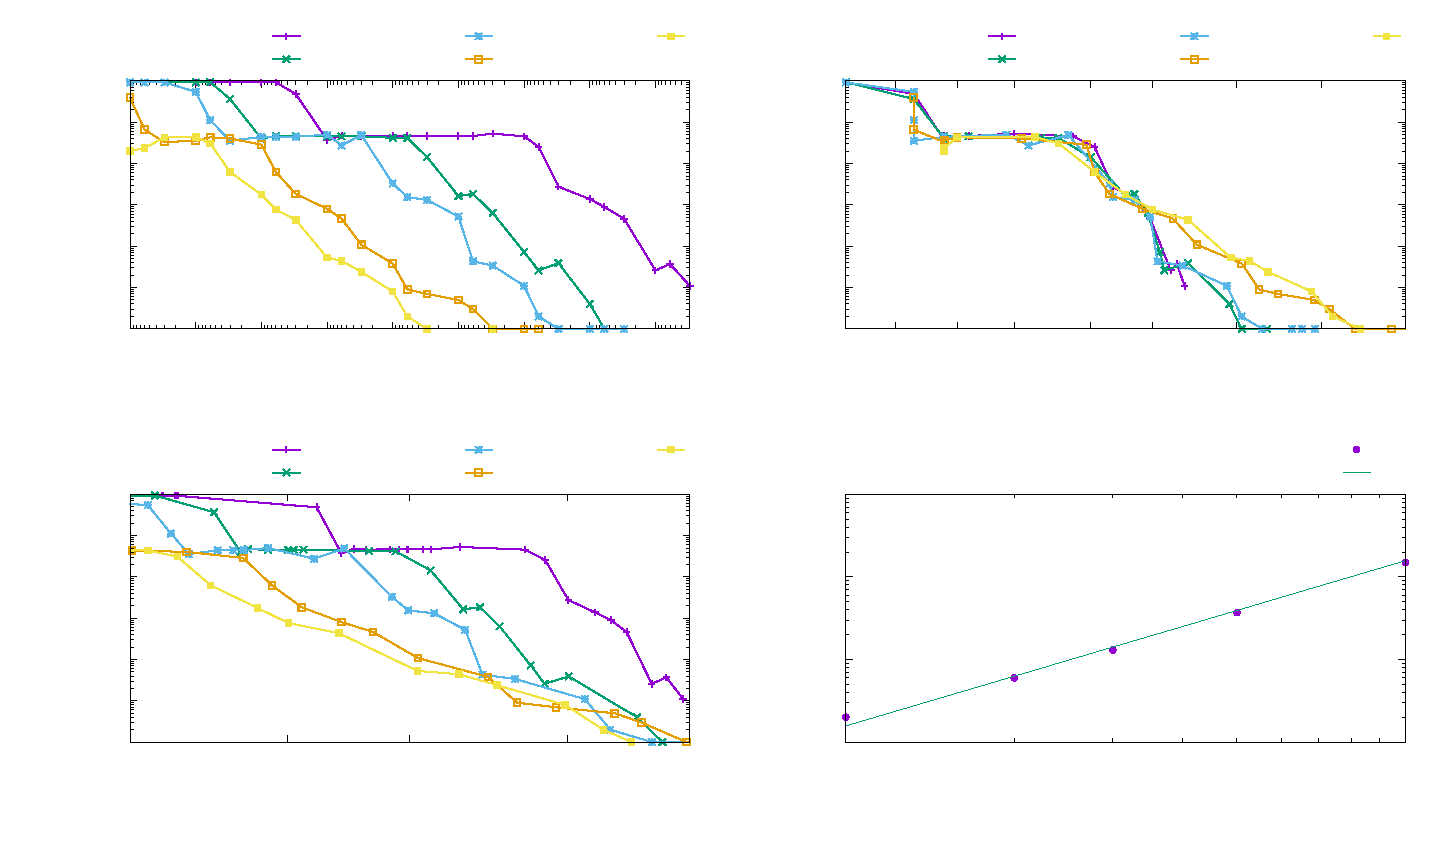
\includegraphics{figS2_1-inc}}%
    \gplfronttext
  \end{picture}%
\endgroup
\end{document}
